%Schriftgröße, Layout, Papierformat, Art des Dokumentes
%\documentclass[sprache=english]%{TUBAFarbeiten}
\documentclass[11pt,twoside,a4paper]{article}
\usepackage[utf8]{inputenc}

%%%%%%%%%
\usepackage{amsmath}
\usepackage{icomma}	%% fuer schoene Kommata
\usepackage{url}	%% um URLs zu setzen und zu verlinken
\usepackage{graphicx,textcomp,booktabs,amsmath}
\usepackage{amssymb,extarrows,cancel,wasysym} %% zusaetzliche mathematische Symbole
\usepackage[scaled]{helvet}
\usepackage{mathptmx,courier} %% Schriftart
\usepackage{microtype} % tolle Typo
\usepackage{lscape} % zur Benutzung von landscape
\usepackage{dcolumn} % fuer schoene Ausrichtung der Tabelleneintr"age
\usepackage{nicefrac} % fuer schoene Brueche im Text
\usepackage{verbatim}
\usepackage{array}
\usepackage{listings} %for source code
\usepackage{setspace} % Um Zeilenabstand zu setzen

%Einstellungen der Seitenränder
\usepackage[inner=3cm,outer=4cm,top=2cm,bottom=3cm,includeheadfoot]{geometry}

%neue Rechtschreibung
\usepackage[english]{babel}

%print CPD and FG-DVC as type
\newcommand{\CPD}{\texttt{CPD} }	% CPD
\newcommand{\FGDVC}{\texttt{FG-DVC} }	% FG-DVC

%Kopf- und Fußzeile
\usepackage{fancyhdr}
\pagestyle{fancy}
\fancyhf{}

%Kopfzeile links bzw. innen
\fancyhead[LO,RE]{\nouppercase{\leftmark}}
%Kopfzeile rechts bzw. außen
\fancyhead[RO,LE]{\thepage}
%Linie oben
\renewcommand{\headrulewidth}{0.5pt}

%Fußzeile links bzw. innen
%\fancyfoot[LO,RE]{Program Controlling CPD and FG-DVC}
%Linie unten
%\renewcommand{\footrulewidth}{0.5pt}

% Title Page
\title{Manual\\\textbf{{PKP}}}
\author{Martin Pollack, Michele Vascellari}

\begin{document}
\maketitle\newpage
\tableofcontents\newpage
\section{User Manual}\label{S_Manual}

PKP, the Pyrolysis Kinetic Preprocessor, is a tool to generate the parameter for modeling the pyrolysis process in CFD-applications. It allows a central data input for all three connected pyrolysis programs \texttt{CPD}, \texttt{CPD} and \texttt{PC Coal Lab}. The results of the selected pyrolysis programs will be used to generate the kinetic parameter for several kinetic models: constant Rate, Arrhenius rate, Kobayashi model and the Distributed Activation Energy Model (DAEM), see chapter~\ref{SS_KinEq}. A second procedure generates parameter for the species and energy balance, chapters~\ref{SSS_ConsEqCPD}~and~\ref{SSS_ConsEqFGDVC}.\\
PKP is written object orientated in Python~2.7.3.

\subsection{First Steps}\label{SS_1stSteps}
Before running the \CPD pyrolysis model with the program the first time, the \CPD-Code\footnote{available at: http://www.et.byu.edu/\texttildelow tom/cpd/cpdcpnlg/cpdcp\_nlgfiles.html} has to be compiled and the executable has to copied to the main directory (containing also the Python code). There the \CPD executable should be renamed \emph{CPD.out}.\footnote{Alternatively the name of the executable can be changed in the \emph{Pyrolysis.py}. But rename the file is the less effort.}
The directory must contain the following files:
\begin{itemize}
 \item Coal.inp (User input for the information about the coal)
 \item CPD.inp (User input for the settings of \CPD)
 \item CPD.out (the \CPD executable)
 \item FGDVC.inp (User input for the settings of \FGDVC)
 \item IN.dat (input file for \texttt{CPD})
 \item OperCond.inp (User input for the operating conditions)
 \item Pyrolysis.py (the main code, accessing to the classes defined in the other *.py)
\end{itemize}
The subdirectory \textit{src} includes the following Python files, \textit{Pyrolysis.py} accesses to:
\begin{itemize}
 \item Compos\_and\_Energy.py
 \item CPD\_Result.py
 \item CPD\_SetAndLaunch.py
 \item FGDVC\_Result.py
 \item FGDVC\_SetAndLaunch.py
 \item FitInfo.py
 \item Fitter.py
 \item InformationFiles.py
 \item Models.py
\end{itemize}
Before running FG-DVC, the directories have to be defined, see the paragraph~\textbf{FGDVC.inp} in chapter~\ref{SS_Generate_Results}. There the  two information for ~\textbf{main directory FG-DVC:} and \textbf{print increment, writeValue:} must be defined. For CPD \textbf{print increment, writeValue:} must be defined. All these information are kept, also when using the GUI as input. So they just have to be defined once as long as they don't need to be changed.

\subsection{Generate Results}\label{SS_Generate_Results}
The output of the pyrolysis programs has to be individually modified for a further work with. Also the user of PKP should be aware of the following points:
\paragraph{FG-DVC}
PKP was tested using \FGDVC version 8.2.3. Also the output of \FGDVC 8.2.2., which seems to be concerning the shape identical to 8.2.3, was tested.
\begin{itemize}
 \item \FGDVC merge the olefins and paraffins into the rate of tar. But the yields of tar, outputted by \FGDVC just consider the species of tar except the olefins and paraffins. As the olefins and paraffins are in general not considered as single species in CFD combustion and gasification applications, the yield of tar generated by \FGDVC further also includes the Olefins and Paraffins. As the output of the olefins and paraffins themselves are correct, the kinetic parameter of this two species are additionally still fitted.
 \item The output of \FGDVC does not directly report the yields and rates of hydrogen. To generate this information, the yields of hydrogen are calculated by subtract the light gases ($CH_4$, CO, $CO_2$, $H_2O$, ...) from the total yields (last column in the 'gasyield.txt'). The rate is gained by derive a smoothed curve\footnote{The subtraction of the other species leads to small oscillation in the yields. These yield curves are further usable. But deriving this curve strengthen this oscillation to a giant value. So the yield curve has to be smoothed before deriving it by apply the equation $y_i=\frac{1}{2} \alpha \cdot (y_{i-1}+y_{i+1})+(1-\alpha) \cdot y_i$ fifty times over all points of the yields. This has still a low influence on the results (applying it very often would lead to a flat curve), but decreases the oscillation that much, that they are small at the derived curve (central differencing scheme).}.
 \item The amount of moisture and ash is both equal zero. This is recommended in the manual. Trying to set a fraction of moisture and ash leads to unrealistic results in the \FGDVC output (negative yields and rates).
 \item The constant numerical time step for \FGDVC defined by the user shouldn't be lower than $10^{-3}$. The temperature history defined by the user is imported by \FGDVC as a text file\footnote{'tTHistory.txt' which was generated by PKP and written into the \FGDVC main directory.}. According to experience can \FGDVC not read imported text files defining the temperature history with a precision better than the $10^{-3}$.
\end{itemize}

\paragraph{CPD}
\begin{itemize}
 \item The outputted result files of \CPD does contain various information. For the further work the fraction of yields~(beginning with 'f', e.g. 'ftar' in the first and fourth \CPD output file are further observed.)
 \item As the \CPD output does not contain the rates, these rates over time are generated by deriving them using the CDS.
 \item If an oscillation in the output of the rates occur is the time step too low. There are not enough counting numbers in the output file. So the reported rates vary from zero (the in the CDS subtracted two yields have the same value) and a very high value (the last counting number changes, but the time step is very low).\\
 The user has here the following possibilities to solve this problem:
 \begin{itemize}
  \item Use a lower time step.
  \item Set '\textit{print increment, writeValue:}' in \emph{CPD.inp} to a high value. The calculation is still carried out with the ow time step. But not every calculated time is written into the result file.
  \item Modify the precision of the \CPD output by modify the \CPD code. If just the number of counting numbers is modified PKP will still be able to read this modified output.
 \end{itemize}
\end{itemize}

The user of PKP can apply a number of runs up to five of the pyrolysis programs. Every runs must have its individual temperature history. The different devolatilization results caused by the different operating conditions shall ensure a better applicability of the kinetics in CFD simulations, where the operating conditions can vary over a range. Taking responsibility to the computational costs, two or three runs is a good option to generate the kinetic parameter.\\

The directly outputted results of the pyrolysis programs are copied into the main PKP directory. The number of the run is contained in the filename.\\

The following subsections give mode detailed information and an overview on the specific user input and the generated PKP results.


\subsubsection{Using the Graphical User Interface}\label{SSS_GUI}
\begin{figure}
\centering
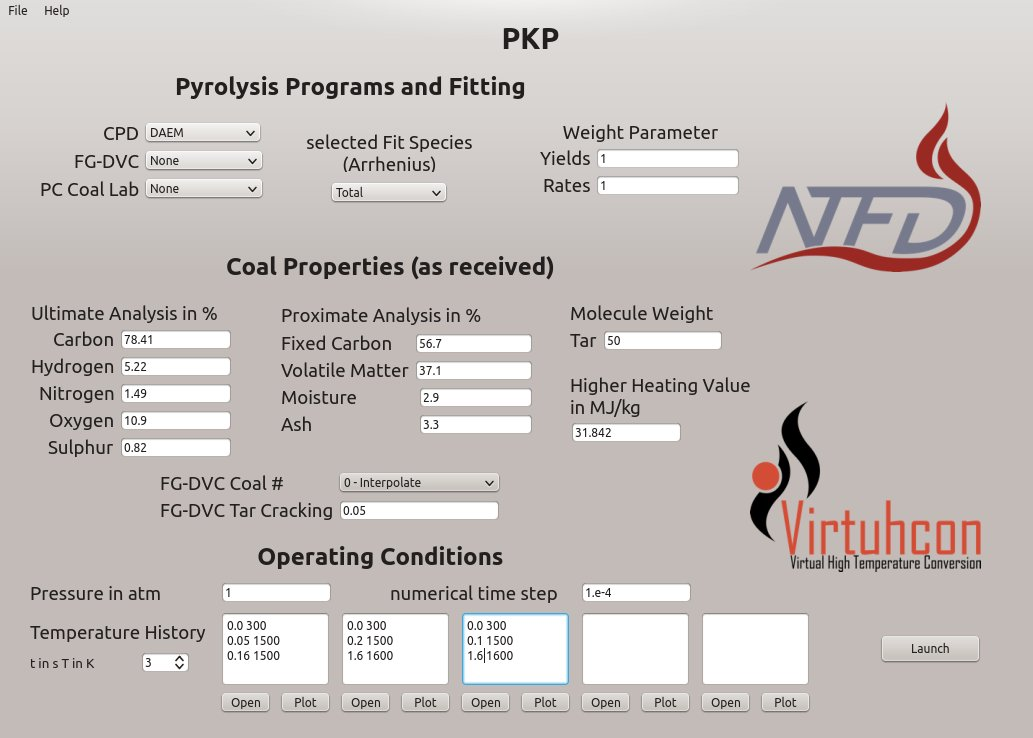
\includegraphics[width=14cm,angle=0]{Figures/GUI}
\caption{A screenshot of the Input GUI.}
\label{F_GUI}
\end{figure}

When starting the graphical user interface, file \emph{PKPgui.py}, the central input windows opens, see figure~\ref{F_GUI}.
As also visible in this figure, the general input structure is splitted into three parts: \emph{Pyrolysis Programs and Fitting}, \emph{Coal Properties} and~\emph{Operating Conditions}. The following selections can be done in the first of these:
\begin{itemize}
 \item \textbf{CPD}, \textbf{FG-DVC}, \textbf{PC Coal Lab}: These column boxes allow a selection, which of these detailed models shall be used and which kinetic parameter shall be fitted. The first two possible selections are here \emph{None}, for not running this model, \emph{Run} to just run it and make the species analysis. A fitting of kinetic parameter will not be carried out. Additional selections for fitting the results are \emph{constant~Rate}~(eq.~\ref{E_Reaction_g}), \emph{Arrhenius}~(eq.~\ref{E_Arrhenius_g}), \emph{Arrhenius~no~B}~(eq.~\ref{E_Arrhenius_g_noB}), \emph{Kobayashi}~(eq.~\ref{E_Kobayashi}) and \emph{DAEM}~(eq.~\ref{E_DAEM}). Here the fitting and the species analysis will be done.
 \item \textbf{selected Fit Species (Arrhenius)} is only important if one of the selected models to fit is \emph{Arrhenius} or \emph{Arrhenius~no~B}. This column box allows which species shall be fitted. Possible options to choose are here:
 \begin{itemize}
  \item \emph{Total}: only the overall yield is fitted
  \item \emph{Main Species}: the yield curves of the overall yields, tar and gas~(the sum of the light gases) are fitted
  \item \emph{all Species}: the kinetic parameter for all species outputted by the detailed model are fitted
 \end{itemize}
 \item \textbf{Weight Parameter} Enter the parameter for the fitting procedure. The text line Weight Parameter Yields sets the factor $\mathrm{a_0}$ in equation~\ref{E_Weight_Param1}, Rates sets $\mathrm{a_1}$ in equation~\ref{E_Weight_Param2}.
\end{itemize}
The second section of the GUI, the information about the coal can be entered. All properties refer to the coal in the as received state.
\begin{itemize}
 \item \textbf{Ultimate Analysis in ~\%} Sets the ultimate analysis of the coal. Values should be in percent.
 \item \textbf{Proximate Analysis in~\%} Sets the proximate analysis of the coal. Values should be in percent.
 \item \textbf{Molecule Weight Tar}: define the molecule weight of the tar. Required for the species analysis.
 \item \textbf{Higher Veating Value} Enter here the higher heating value of the coal in $\mathrm{\frac{MJ}{kg}}$.
 \item \textbf{FG-DVC Coal \#} FG-DVC needs an information whether the coal property file should be interpolated using the van-Krevelen~Diagram (option \emph{0-Interpolate}) or if a library coal should be used (1-8). If the selected coal is out of the range of the library coals, the closest library coal has to be selected. The generation of the coal file is also done automatically by PKP.\footnote{Using the FG-DVC \emph{coalsd.exe}. For more information see the FG-DVC manual.}
 \item \textbf{FG-DVC tar cracking} Defines the FG-DVC modeling of the tar cracking. Possible selections are:
 \begin{itemize}
  \item \emph{0.0} No tar cracking is modeled.\footnote{The option recommended by the FG-DVC manual~\cite{FGDVC_822}.}
  \item When entering a time in seconds, e.g. '0.01', defines the holding time of the tar in the coal molecule. The tar is cracked during this time frame.
  \item A negative number, e.g. '-1', sets the full tar cracking.
 \end{itemize}
\end{itemize}

The last section in the GUI allows the input of the operating conditions:
\begin{itemize}
 \item \textbf{Pressure in atm} Defines the pressure where the devolatilization occurs.
 \item \textbf{numerical time step} Sets the time step. For FG-DVC the constant value, for CPD the maximum.
 \item \textbf{Temperature History} With the spin box on the left, the numbers of temperature histories to apply is defined. If this is set to '3', three runs are carried out using the first three temperature histories. These temperature histories can be imported via the five text fields on the right. There the temperature histories can be entered manually or also be imported using the 'open' buttons in below. Additionally they can be plotted (button 'plot'). Using this option also saves the temperature history in a file~\emph{TempHist1.dat}.Where the number stands for the current field. These saved temperature histories can be re-imported using the 'open' button.\\
 All the temperature histories have to be entered in two columns, just separated by spaces. The time is in seconds, the temperature in Kelvin.
\end{itemize}

The head menu contains under File following options:
\begin{center}
\begin{tabular}{ll}
Write into Table & Ctrl+S\\
Write and Run & Ctrl+R\\
Load saved state & Ctrl+O\\
Show generated Results & Ctrl+T\\
Exit & Ctrl+Q\\
\end{tabular}
\end{center}
Where the Write saved all information into the \emph{.inp} files and the \emph{TempHist\#.dat} in the main directory. 'Load saved state' transfer this information into the current GUI.\\
The 'Write and Run' is identical with the button 'Launch' in the lower right of the GUI.\\
The file menu 'Help' offers to open this manual.\\

Please do not forget to make the general settings in the input files, before using PKP the first time, see chapter~\ref{SS_1stSteps}.\\

After running the result windows opens, figure~\ref{F_GUIDone}. It lists all calculated species in the column bar. With 'Show results' the yields over time for the detailed model output and the fitted equation are plotted. 'Open Species analysis' opens the textiles with the species analysis results for each run. Open kinetic parameter opens the text file with the results of the fitting, one file for each detailed model. If this window was closed, it can be reopened by the option 'Show generated Results'~(Ctrl+T) in the Main window. \\
All results are located in the Result directory. When starting a new run, its content is deleted.\\

\begin{figure}
\centering
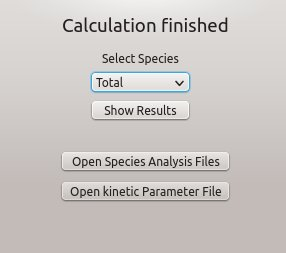
\includegraphics[width=4cm,angle=0]{Figures/GUI_Done}
\caption{A screenshot of the Result GUI.}
\label{F_GUIDone}
\end{figure}

\subsubsection{Using the input files}\label{SSS_inp}
The manual user input is managed by the four \emph{*.inp} files, \emph{Coal.inp, CPD.inp} \emph{FGDVC.inp} and \emph{OperCond.inp}.\\
The information you want to insert into these files have to be in the line below the line asking for the information. For example:\\

\noindent \emph{Fixed Carbon:\\
43.7}\\

This sets the amount of Fixed Carbon equal 43.7. The position~(i.e. the line) of such two lines in the input file does not matter, the only important point is the specific string~(in this example~\emph{Fixed Carbon:}) and that the value you want to set is in the following line after the string.\footnote{If you want to use another string in this file, you also have to change the individual file note in \emph{InformationFiles.py}.}\\
Firstly you will get a short overview into these files and the values to enter into them:\\
\paragraph{Coal.inp} contains the main information about the coal. PKP forwards the information about the coal from this file to the programs \CPD and the \FGDVC coal generator (\textit{/COALS/coalsd.exe} in the \FGDVC directory). The proximate analysis values are only required by \texttt{CPD}.
\begin{itemize}
 \item \textbf{Fixed Carbon:} sets the amount of fixed carbon in the coal. The value has to be entered in percent for a non-daf coal.
 \item \textbf{Volatile Matter:} sets the amount of volatile matter in the coal in percent, as received.
 \item \textbf{UA Carbon:}, \textbf{UA Hydrogen:}, \textbf{UA Nitrogen:}, \textbf{UA Oxygen:} sets the ultimate analysis for the coal to model. The values have to be entered in percent.
 \item \textbf{Higher Heating Value, as received, in J/kg:} sets the higher heating value for the coal. If this value is not known, set it equal zero. Then the Dulong formula~(equation~\ref{E_Dulong}) will be used to calculate the higher heating value.
 \item \textbf{Tar Molecule weight, MTar:} Sets the molecule weight of the tar, as it is required for the species and energy calculation, see chapters~\ref{SSS_ConsEqCPD}~and~\ref{SSS_ConsEqFGDVC}.
 \item \textbf{Weight-Parameter yields for fitting the kinetics:} sets the weight $\mathrm{a_0}$ of the equation~\ref{E_Weight_Param1} to weight the yields in the fitting procedure~(equation~\ref{E_LS}).
 \item \textbf{Weight-Parameter rates for fitting the kinetics:}  sets the weight $\mathrm{a_1}$ of the equation~\ref{E_Weight_Param2} to weight the rates in the fitting procedure~(equation~\ref{E_LS}).
\end{itemize}

\paragraph{CPD.inp} controls the \CPD program and the further work with its output.
\begin{itemize}
 \item \textbf{useCPD?:} if set to \emph{yes} or \emph{true}, \CPD will be launched.
 \item \textbf{selected fitting Approximation:} if the \emph{constantRate} is selected, the fitting will be carried out using equation~\ref{E_constRate_s}~and~\ref{E_constRate_g}. When selecting \emph{Arrhenius}, the kinetic parameter for the Arrhenius equation modeled pyrolysis kinetics~(equation~\ref{E_Arrhenius_g}) will be calculated. To fit the Kobayashi parameter, set it to \emph{Kobayashi}. If selecting \emph{None}, no fitting of the kinetic parameter will be carried out, just the direct \CPD results and species and energy balance will be generated.
 \item \textbf{initial time step in s:} The initial time step, \CPD starts to calculate with.
\item \textbf{print increment, writeValue:} Integer which sets the frequency of writing the result into the \texttt{CPD}-output file. E.g. '1' means every value is written into the file, '3' only every third value.
\end{itemize}

\paragraph{FGDVC.inp} controls the \FGDVC program and the further work with its output.
\begin{itemize}
 \item \textbf{use FG-DVC?:}  if set to \emph{yes} or \emph{true}, \FGDVC will be launched.
 \item \textbf{selected fitting Approximation:} This selection is analogous to the in \textit{CPD.inp}
 \item \textbf{main directory FG-DVC:} sets the main path of \texttt{FG-DVC}, where the \emph{fgdvc.exe} is located. One example: '{C:\verb|\|Programs\verb|\|FGDVC\_8-2-3\verb|\|}'
 \item \textbf{directory fgdvc-output:} Sets the main directory, where \FGDVC outputs the results. This is in general the directory, where the \emph{fgdvcd.exe} is located. One example: '{C:\verb|\|Programs\verb|\|FGDVC\_8-2-3\verb|\|FGDVC\verb|\|}'.\\To use other already generated FG-DVC output files, it is a good option to set their path here. As long as they are still named \emph{gasrate.txt} and \emph{gasyield.txt}, the fitting will be carried out on the information contained in these files.
 \item \textbf{Choose Coal:} If this is set equal \emph{0}, the interpolation of the coal will be carried out using the information from \emph{Coal.inp} and the FG-DVC program \emph{coalsd.exe}, leading to specific \FGDVC coal files for the applied coal. If the file cannot be generated, i.e. the used coal is outside the interpolation triangle\footnote{see the FG-DVC manual for more details: THE FG-DVC COAL PYROLYSIS MODEL USER'S GUIDE Version 8.2.3 for Windows; Advanced Fuel Research, Inc., 87 Church Street, East Hartford, CT 06108-3728, USA; 2012}, select a value from \emph{1}~to~\emph{8} to use one of the \FGDVC library coals. The order here is the same as in \texttt{FG-DVC}:
 \begin{enumerate}
  \item Beulah-Zap
  \item Wyodak-Anderson
  \item Illinois \# 6
  \item Bind Canyon, UT
  \item Lewis-Stockton, WV
  \item Pittsburgh \# 8
  \item Upper Freeport, PA
  \item Pocahontas \# 3, VA
 \end{enumerate}
 \item \textbf{Model tar cracking?} To model no tar cracking~(as recommended in the \FGDVC manual) set the tar residence time equal \emph{0}. A partial tar cracking can be modeled by set the tar residence time is seconds. If a full tar cracking shall be used, set the residence time to a negative input value, e.g write \emph{-1}.           
\end{itemize}

\paragraph{OperCond.inp} sets the operating condition for the pyrolysis programs.
\begin{itemize}
  \item \textbf{pressure in atm:} Sets the constant pressure in atmospheres.
 \item \textbf{FG-DVC: constant (numerical) time step; CPD: maximum time step}: Enter here the numerical time step, the constant for \FGDVC and the maximum value for \texttt{CPD}.
 \item \textbf{Number of Temperature Histories to include:} Defines, how many runs of the pyrolysis  models should be carried out. The different temperature history will be defined with the help of the next point:
 \item \textbf{Start Time History 1:} This line have to follow two columns, defining the temperature history for the first run of the pyrolysis models. The first column lists the time in seconds, the second one the temperature in K. The last time point is automatically selected as the final pyrolysis time. The end of the time-temperature array has to be labeled by the term \emph{End Time History 1}. Here one example:\\
\emph{Start Time History 1\\
0, 293\\
0.05, 1000\\
0.1, 1700\\
0.6, 1700\\
End Time History 1\\}
Analogue to this term the numbers 2~to~5 label the temperature history for the second to the fifth run.
\end{itemize}


\subsubsection{The Result Files}\label{SSS_ResultsFiles}
The generated results are documented in the following files. The name of the text-files contains in front the used pyrolysis program (e.g. \emph{CPD-BalanceResults.txt}).

\paragraph{BalanceResults.txt}
This file contains the output of the species and the energy conservation, chapters~\ref{SSS_ConsEqCPD}
~and~\ref{SSS_ConsEqFGDVC}. The first part lists the input of the UA, PA and HHV. Afterwards, the final yields of all species are enumerated, as the result of using the equation~\ref{E_add_up}~to~\ref{E_MethanNew}. The tar composition~(equation~\ref{E_TarComp}), assuming a $\mathrm{C_nH_mO_p}$ molecule with an average molecule mass, inputted by the user, is given by the factors n, m, p. The last two parts show the results applying the equations~\ref{E_Dulong}~to~\ref{E_QPyro}.

\paragraph{Results\_const\_rate.txt}
This file contains the kinetic parameters for the constant rate (equation~\ref{E_constRate_s}~or~\ref{E_constRate_g}) fitting. The two parameters are k in $\mathrm{\frac{1}{s}}$ and $\mathrm{t_{start}}$ in s.

\paragraph{Result\_ArrheniusRate.txt}
\emph{Result\_ArrheniusRate.txt} lists all kinetic parameter~(A in $\mathrm{\frac{1}{s}}$ and E~in~K) for the Arrhenius equation~\ref{E_Arrhenius_s}~or~\ref{E_Arrhenius_g}.

\paragraph{Results\_KobayashiRate.txt}
This file list for all species the Kobayashi kinetic parameter $\mathrm{A_1 \; and \; A_2 \; in \; \frac{1}{s}}$, $\mathrm{E_1 \; and \; E_2 \; in \; K}$, $\mathrm{\alpha_1 \; and \; \alpha_2}$.

\paragraph{Fit\_result\_[Species]\_[R/Y].pdf}
These files contains the plots of the pyrolysis program output curve and the estimated curve using the applied model. These plots show the rate (then *\_R.pdf) or yields (*\_Y.pdf). This plot exists for all species calculated by the pyrolysis program (named in *\_Species\_*).

\paragraph{Fit\_result\_[Species].out}
For every species is in the referring file the \emph{Time}, \emph{Temperature}, \emph{Yields} and the \emph{Rates} written in columns. This is not the original output from the pyrolysis program, it is the result applying the selected equation with the fitted parameter.

\section{Programs Structure}\label{S_Program}
The files, the directory must contain, are listed in chapter~\ref{SS_1stSteps}. The python code is written in the files  \emph{CPD\_Compos\_and\_Energy.py}, \emph{CPD\_Fit\_lin\_regr.py}, \emph{CPD\_Fit\_one\_run.py} and \emph{Pyrolysis.py}. The last enumerated file controls the whole process. It accesses to the other three files, which contain the corresponding classes with their methods.\\
The figure~\ref{F_Structure} gives a overview of the program structure.\\

proximate analysis~(PA), the ultimate analysis~(UA), both in percent, and the higher heating value~(HHV)

\begin{figure}
\centering%\capstart
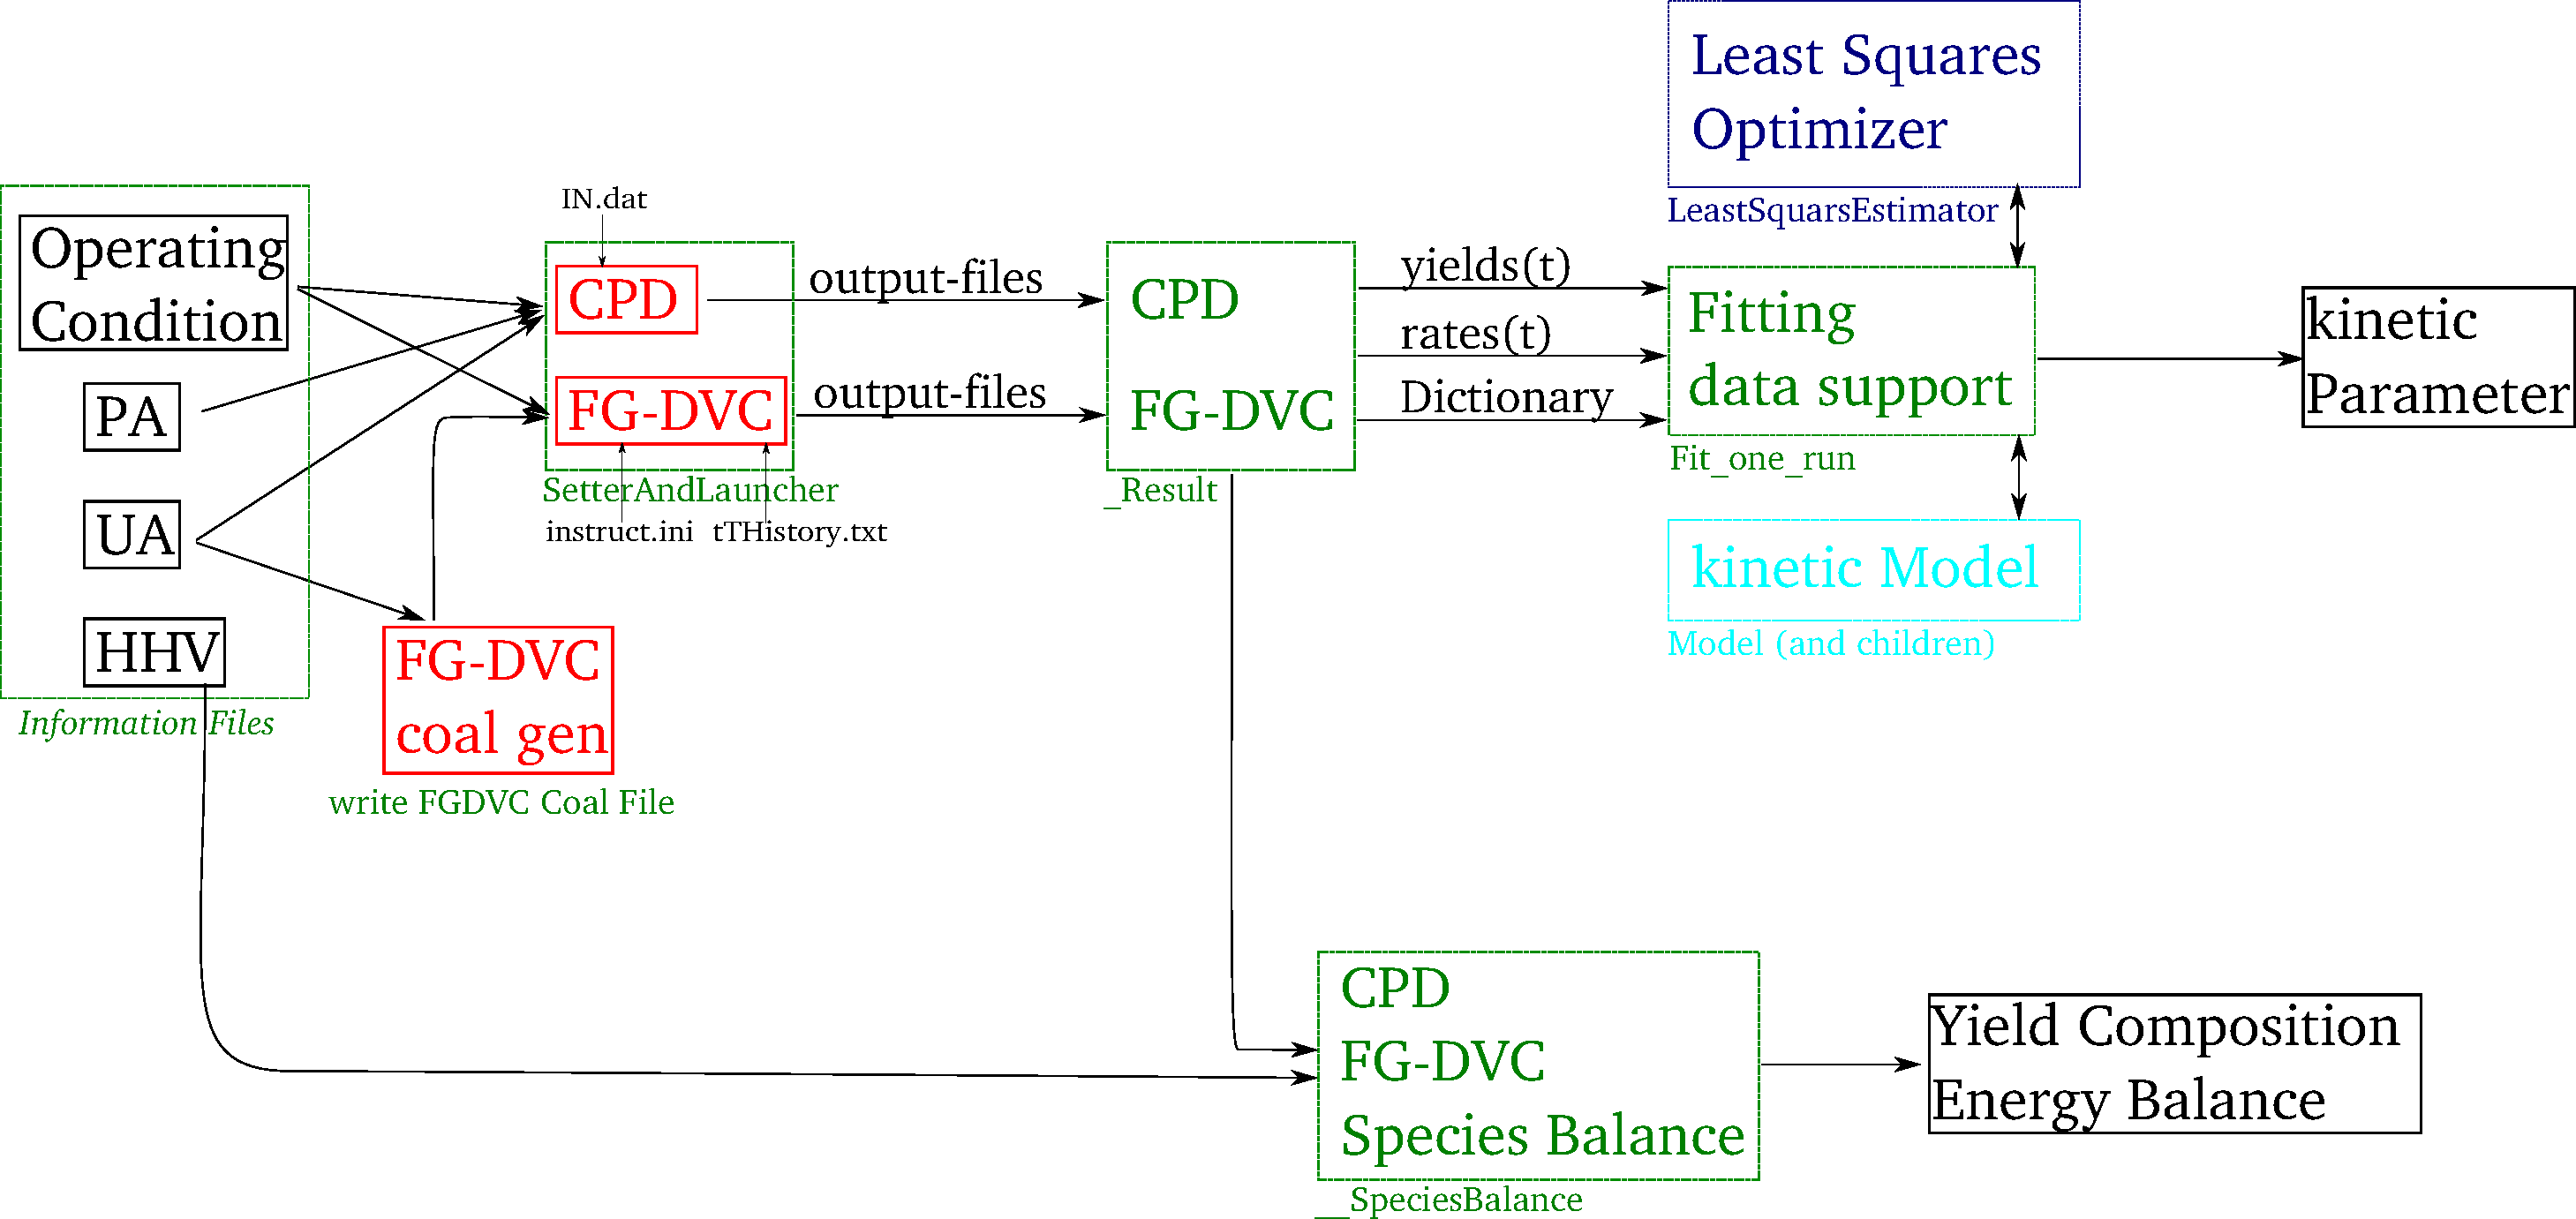
\includegraphics[height=6cm,angle=90]{Figures/Programstructure}
\caption{Overview of the program}
\label{F_Structure}
\end{figure}

\_Result class supports other classes with whole yields and rates Arrays and dictionaries\\
-Dict makes Porgram better to read ('Temp' instead of colnr) and more robust against changes (if another colnr all cols in program had to be changed)\\
-Dict needs only be changed in \_Result\\
-other classes independent from CPD/FG-DVC\\
\newpage
\bibliographystyle{plain}%plain, abbrv, alpha
\bibliography{bibo}
\end{document}
